\documentclass[proseminar,german,utf8]{zihpub}
\usepackage{setspace}
\usepackage{hyperref}
\usepackage{graphicx}

\author{Paul Gottschaldt}
\title{Julia - High-Performance Programmiersprache für High-Performance Computing?}
\matno{4609055}
\betreuer{Martin Schroschk}
\bibfiles{references}
\copyrighterklaerung{Hier soll jeder Autor die von ihm eingeholten
Zustimmungen der Copyright-Besitzer angeben bzw. die in Web Press
Rooms angegebenen generellen Konditionen seiner Text- und
Bild\"ubernahmen zitieren.}
\acknowledgments{Die Danksagung...}

\begin{document}

Das ist eine Referenz auf Klein~\cite{blackholes}. Die Referenzliste ist in der Datei references.bib definiert.

\section {Einleitung}
1998 startete das Apache-Point-Observatorium in New Mexico ihr Projekt Sloan Digital Sky Survey (SDSS), welches Fotos von über 35~\% aller sichtbaren Objekte unseres Himmels anfertigte und in einer Datenbank zunächst sicherte. Seit diesem Jahr wurden bereits über 500 Millionen Sterne und Galaxien fotografiert und Licht eingefangen, welches bereits Milliarden von Jahren unterwegs war und uns bis weit in die Vergangenheit unseres Universums zurückblicken lässt. Die SDSS Kamera galt als produktivste Weltraumkamera der Welt bis zu ihrer Abschaltung im November 2009. Mit etwa 200 GB reine Bilddaten pro Nacht entstand so eine Datenbank mit über 5 Millionen Bildern von jeweils 12 Megabyte - zusammengerechnet also rund 55 Terabyte\footnote{\url{https://juliacomputing.com/press/2016/11/28/celeste.html}}. 2014 startete ein Team von Astronomen, Physikern, Informatikern und Statistikern das Projekt Celeste um eben jenen Datensatz zu katalogisieren und für jeden Himmelskörper einen Eintrag anzulegen\footnote{\url{https://juliacomputing.com/case-studies/celeste.html}}. In der ersten veröffentlichten Version von 2015 noch auf Berechnungen auf einzelne Knoten beschränkt, schaffte es das Forschungsteam um die involvierten Parteien Julia Computing, UC Berkeley, Intel, National Energy Research Scientific Computing Center (NERSC) und Lawrence Berkeley National Laboratory in der 2. Version von 2016 bereits einen 225-fachen Geschwindigkeitsgewinn zu erzielen. Die größten Verbesserungen waren dabei der mit 8192 Intel® Xeon® Prozessoren ausgestattete HPC des Berkeley Lab's und Julia, eine High-Performance Open-Source Programmiersprache, die bis dato noch relativ unbekannt war und seit 2009 am MIT entwickelt wird. Besonders ist an Julia vorallem ihr Anspruch, eine sehr produktive (high-programming language) wie Python zu sein, dabei aber Geschwindigkeiten wie C zu erreichen. Im November 2017 veröffentlichte dieses Team dann die aktuelle 3. Version, mit der sie nochmals einen deutlichen Geschwindigkeitsgewinn erreichen konnten. Sie schafften es 188 Millionen Sterne und Galaxien in nur 14.6 Minuten zu katalogisieren und nutzten dafür bis zu 1.3 Millionen Threads auf den 9300 Knights Landing(KNL) Knoten des Cori Supercomputers des NERSC. Dabei erzielten sie mit Julia eine Peak-Performance von 1.54 PetaFlop/s für Gleitkommaberechnungen mit doppelter Genauigkeit. Damit erzielt das Celeste Projekt einen 100-fachen Gewinn zu allen vorherigen Forschungsprojekten. Derzeit gibt es rund 200 Supercomputer in der Welt, welche in der Lage sind eine Peak-Performance von mehr als einem Petaflop pro Sekunde zu erreichen. Trotzdem sind so gut wie alle Anwendungen, welche eben jene Peak-Performance erreichen von einer Gruppe von Ninjas geschrieben, welche ein sehr tiefes Verständnis für alle erforderlichen Details besitzen, die man benötigt um solch eine Performance zu erreichen\footnote{\url{https://www.nextplatform.com/2017/11/28/julia-language-delivers-petascale-hpc-performance/}}. Umso erstaunlicher ist an diesem Ergebnis also die Tatsache, dass das Team hinter Celeste ihre Geschwindigkeit ausschließlich unter Nutzung ihrer Kenntnisse, dem Juliacode und dessen Threading Model erzielen konnten.

\begin{figure}[hbt!]
  \centering
  \caption{Eine Abbildungsbeschreibung}
  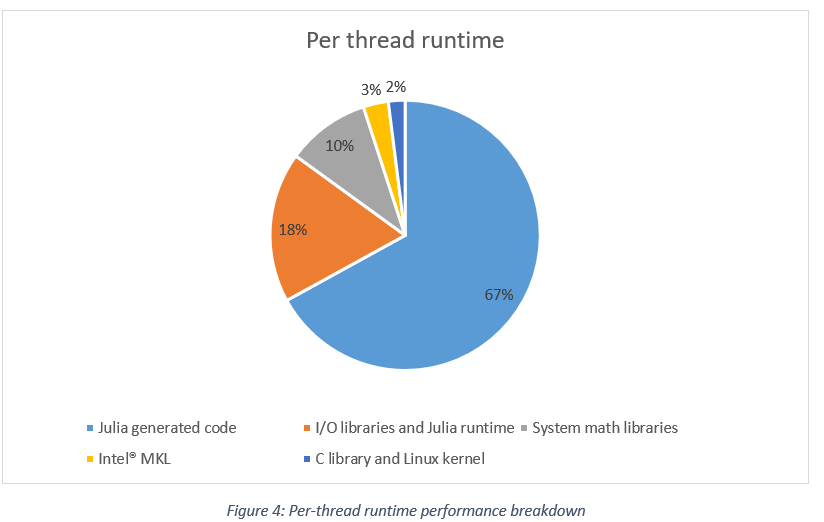
\includegraphics[scale=0.5]{celestejulia.png}
  \label{fig:celestejulia}
\end{figure}

Wie in der Abbildung~\ref{fig:celestejulia} zur pro Thread Auslastung zu sehen, lieferte Julia 82.3\% der Performance. Damit stellt Julia unter Beweis das es sowohl für ThetaByte-große Datensätze, wie auch für PetaByte-schnelle Berechnungen geeignet ist. Keno Fischer, CTO von Julia Computing, sagte 2017, das Projekte wie Celeste unter Beweis stellen, das der Traum, der hinter Julia steht, wahr wird. Wissenschaftler können nun auf ihrem Rechner entwickelte Prototypen einfach von ihrem Laptop auf die größten Supercomputer verschieben ohne zwischen Sprachen wechseln zu müssen oder ihren Code gar komplett neu zu schreiben. Sie (Anmerkung: Entwickler von Julia Computing) sind sehr stolz darauf, dies alles geschafft zu haben und glauben sehr daran, das Julia die Entwcklung in der Forschung für viele Jahre sehr voranbringen wird. Viral Shah, CEO von Julia Computing, sagte das Forscher sich nun auf die Lösung ihrer Probleme fokussieren können und sich nicht mehr mit dem Programmieren beschäftigen müssen\footnote{\url{https://juliacomputing.com/press/2016/11/28/celeste.html}}.
%%%%%%%%%%%%%%%%%%%%%%%%%%%%%%%%%%%%%%%%%%%%%%%%%%%%%%%%%%%%%%%%%%%%%%%

\section{Einführung in die Programmiersprache Julia}
\subsection{Julia, die dynamische, stark typisierte funktionale Programmiersprache}
Julia ist eine junge, flexible, höhere Programmiersprache die es sich selbst als Ziel gesetzt hat, die hohe Produktivität und einfache Handhabbarkeit aus Sprachen wie Python mit der Geschwindigkeit von C zu kombinieren. Auch wenn sie vorallem für wisssentschaftliches und numerisches Programmieren gestaltet worden ist, bietet sie eine sogleich performante wie auch einfach zu lernende Umgebung und versucht damit den derzeitigen Trend von mehrsprachigen Softwarelösungen in der Wissenschaft entgegen zu wirken. Mit einem Syntax der an eine Kombination aus MATLAB und Python erinnert, Lisp ähnlichen Macros und Metaprogrammierung, einem Compiler der LLVM nutzt und einem eigenem Paketmanager der an Git erinnert, hat sich Julia viele bereits etablierte Funktionen zunutze gemacht. Zusätzlich besitzt sie die Möglichkeit C und Python Funktionen einfach direkt aufzurufen was die Nutzung der Bibliotheken der beiden Sprachen direkt im Julia Code ermöglicht. Julias gute Performance wird vorallem durch Multimethoden für einzelne Funktionen und die automatische Generierung von effizientem typspezialisierten Code gewonnen. Dabei ist Julia sowohl dynamisch wie auch statisch typisiert. Zudem ist Julia funktional, objektorientiert und imperativ und wurde fast komplett in Julia selbst geschrieben.
%%%%%%%%%%%%%%%%%%%%%%%%%%%%%%%%%%%%%%%%%%%%%%%%%%%%%%%%%%%%%%%%%%%%%%%
\subsection{Julias Typensystem und Multimethoden}

In Julia gibt es keine Klassen wie es sonst für objektorientierte Sprachen üblich ist. Stattdessen trennt Julia explizit die Daten eines Objekts von dessen Methoden.Vom Nutzer angelegte Objekte wie sie aus anderen puren objektorientierten Sprachen wie C++ oder Java bekannt sind ähneln am meisten dem Composite Types. Auch bekannt unter Namen wie struct oder records stellt er eine Ansammlung von benannten Feldern da. Diese einzelnen Felder können wie einzelne Attribute betrachtet werden und besitzen einen Wert. Wie es der Name auch schon andeutet, ist es möglich diesen Composites ineinander zu schachteln. Zusätzlich erzeugt Julia standartmäßig für jeden Composite Type auch Konstruktoren. Auch wenn Julia dynamisch ist und damit der Typ nicht angegeben werden muss, besitzt jeder Wert einen festen Datentyp, dies gilt auch für die vom Nutzer erstellten Typen. Dabei sind alle Datentypen Laufzeittypen, das heißt den einzigen Datentyp den ein Wert besitzt, ist sein wirklicher aktueller Typ, während das Programm läuft. Auch besitzen nur Werte einen Typ, eine Variable stellt lediglich einen Namen gebunden an einen Datentyp dar. Julias Rückgrat für sein Typensystem sind die abstrakten Datentypen. Während ein Wert immer einen konkreten Datentyp besitzt, ist dieser Typ gleichzeitig in einen Graphen von abstrakten Typen eingebunden. Konkrete Typen sind die Knoten dieses Graphen und können keine Elternknoten sein. Abstrakte Typen dagegen können mehrere Kinder- und Elternknoten besitzen und bilden die Basis von Julia. Der Datentyp Int64 ist zum Beispiel Kindknoten vom abstrakten Typ Signed, welcher Kindknoten vom Typ Integer ist. Als oberster Knoten steht der Datentyp Any, welcher kein Kindknoten ist. Ein Nutzer kann seine definierten Objekte in diesen Graphen einfügen, wenn er nichts weiter spezifiziert wird das Objekt standartmäßig als Kind vom Typ Any angenommen. Als ein weiteres Feature unterstützt Julia zusätzlich auch parameterizierte Datentypen. Diese ermöglichen die generische Erstellung von vielen weiteren kombinierten Datenypen und dienen zudem unterstützend für Julias weiteres Schlüsselmerkmal \-  die Multimethoden. Um Multimethoden zu verstehen, muss zuerst der Syntax von Methoden und Funktionen in Julia geklärt werden. Im Kontext von Julia stellen Funktionen ein Objekt dar, welches ein Tuple von Eingangswerten einem Rückgabewert zuordnet oder eine Fehler wirft. Eine einzelne Funktion fasst dabei einen Sachverhalt wie zB die Addition von Werten zusammen und besitzt unterschiedlich viele verschiedene Methoden, welche je nach Anzahl der Argumente und Typ jedes einzelnen Wertes gewählt wird. Deshalb werden Funktionen in Julia auch generisch genannt. Methoden widerrum sind nun eine explizite Implementierung einer Funktion und werden nach dem Multimethoden-Verfahren (in Englisch multiple dispatch) ausgewählt. Damit grenzt sich Julia im Sinne des objekt-orientierten Paradigmas sehr von Sprachen wie Java oder C++ ab. Während in diesen Sprachen eine Zuordnung nach dem Typ des ersten Arguments (single dispatch) implizit entschieden wird (zB etwas wie obj.meth(arg1,arg2)) werden Methoden in Julia explizit nach dem am exaktesten passenden Argumenttypen (zB etwas wie meth arg1::Int64,arg2::Number) ausgewählt. Am exaktesten passenden Typ meint hier das vom konkreten Typ des Eingabewertes aufsteigend der Typenbaum abgegangen wird, bis eine Methode gefunden wurde, die der Anzahl der Argument und deren Typen entspricht. Wird keine gefunden, so wird ein Fehler geworfen. Multimethoden kombiniert mit den Trennen der Funktionen von den Objekten, auf denen sie arbeiten und dem Typenbaum, ergibt damit eine Art Vererbung die je nach Eingabetypen einer Funktion Verhalten weiterreicht und dabei die Struktur ignoriert. Die Entwickler von Julia selbst sagen, das sie festgestellt haben, das die ledigliche Vererbung von Verhalten unter Ausgrenzung der Struktur bestimmte Schwierigkeiten der objekt-orientierten Sprachen lösen konnte ohne große Nachteile festzustellen. Dies ergibt sich daraus, das Mehrfachvererbung auf konkreten Typen zu einer Hierarchie führt, welche sich nicht gut auf die Wirklichkeit mehr abbilden lässt und auch allgemein alles viel mehr verkompliziert wie man zB am Diamant-Problem gut erkennen kann. Julia hat sich explizit dagegen entschieden, in ihr würde jeder konkrete Typ einem seperaten Blattknoten zugeordnet werden und Typen mit ähnlichen Eigenschaften unter einem abstrakten Typ zusammen gefasst werden.
%%%%%%%%%%%%%%%%%%%%%%%%%%%%%%%%%%%%%%%%%%%%%%%%%%%%%%%%%%%%%%%%%%%%%%%
\subsection{Metaprogrammierung, eine Hommage an Lisp}

Ein weiteres wichtiges Merkmal, das Julia ausmacht, ist seine Unterstützung für Metaprogrammierung. Wie in Lisp, representiert Julia seinen eigenen Code als Datenstruktur in sich selbst. Da dieser Code durch Objekte dargestellt wird, kann er genauso aus Julia heraus auch erstellt und manipuliert werden. Dadurch wird es möglich Code zu transformieren oder gar Code zu generieren. Julia repräsentiert zudem alle Datentypen und den Code in Strukturen, welche in Julia implementiert worden sind, wodurch auch eine sehr mächtige Rückschau (engl. Reflection) möglich ist. Ein Ausdruck wird dabei immer in ein \"Expr\"- Objekt übersetzt, welches sowohl den Typ des Ausdrucks wie auch seine Argumente beinhaltet und in Julia sehr einfach zu bearbeiten oder auszuwerten ist. Dem Datentyp Symbol wird hierbei noch eine sehr bedeutende Rolle zugedacht. Er repräsentiert alle Variablen und damit verbunden auch Zuweisungen und Funktionsaufrufe. In einer Sprache, in der alles durch Objekte intern dargestellt werden kann ist es unabdingbar einen solchen Symbol-Typ zu haben, da es sonst nicht möglich wäre Daten wie Strings von einer Variablen zu unterscheiden. Julia besitzt auch Lisp-ähnliche Macros. Dies sind Funktionen, welche einen Ausdruck als Argument nehmen, ihn manipulieren oder zusätzlichen Code hinzufügen und dann eine Ausdruck zurückgeben. Der Unterschied neben dem \@- mit dem ein Macro beginnt ist vorallem der Zeitpunkt zu dem ein Macro ausgewertet wird. Es wird ausgeführt wenn der Code übersetzt wird und bieten damit die ideale Möglichkeit Funktionen zusätzlich zu manipulieren. Ein gängiges später noch sichtbares Beispiel wäre hier das \@Benchmark Macro welches Performanztests ausführt und mir am Ende neben dem Ergebnis auch die Laufzeit, die Allokationen und den benötigten Speicher für die Funktion zurückgibt. Um die Erstellung und Manipulation von Ausdrücken zu vereinfachen gibt es zudem die Funktion, eine Variable in den Ausdruck im Nachhinein einzufügen. Dies nennt sich zu englisch \"splicing\" oder \"interpolating\" und ist auch für Macros sehr nützlich, da so auch lokale Variablen in Macros übergeben werden können, welche sonst innerhalb des Macros undefiniert werden um Hygiene, also das versehentliche Übernehmen oder Überschreiben von Variablen, zu verhindern.
%%%%%%%%%%%%%%%%%%%%%%%%%%%%%%%%%%%%%%%%%%%%%%%%%%%%%%%%%%%%%%%%%%%%%%%
\subsection{JIT und LLVM}

\section{Parallele Programmierung mit Julia}
\section{Bewertung der HPC-Eignung von Julia}
\section{Quellen}
\subsection{Links}
Links für die Einleitung:
\begin{itemize}
\item https://juliacomputing.com/case-studies/celeste.html am 14.05.18 um 14:52 Uhr
\item https://www.heise.de/developer/meldung/Programmiersprache-Julia-profiliert-sich-beim-High-Performance-Computing-3518621.html am 14.05.18 um 14:52 Uhr
\item https://github.com/jeff-regier/Celeste.jl am 14.05.18 um 14:52 Uhr
\item https://www.youtube.com/watch?v=uecdcADM3hY am 14.05.18 um 14:52 Uhr
\item https://juliacomputing.com/press/2016/11/28/celeste.html am 14.05.18 um 14:52 Uhr
\item https://de.wikipedia.org/wiki/Sloan\_Digital\_Sky\_Survey am 14.05.18 um 14:53 Uhr
\item https://de.wikipedia.org/wiki/Apache\-Point\-Observatorium am 14.05.18 um 14:53 Uhr
\item http://www.astronews.com/news/artikel/2014/01/1401-013.shtml am 14.05.18 um 14:54 Uhr
\item http://www.sdss.org/dr14/imaging/ am 14.05.18 um 14:54 Uhr
\item https://www.nextplatform.com/2017/11/28/julia-language-delivers-petascale-hpc-performance/ am 14.05.18 um 14:54 Uhr
\end{itemize}

Links für die Definition:
\begin{itemize}
\item https://julialang.org/ am 14.05.18 um 14:57 Uhr
\item https://www.heise.de/developer/artikel/Funktionsorientiert\-und\-schnell\-Die\-Programmiersprache\-Julia\-3793160.html?seite=all am 14.05.18 um 14:58 Uhr
\item https://de.wikipedia.org/wiki/Julia\_\(Programmiersprache\) am 14.05.18 um 14:58 Uhr
\item https://docs.julialang.org/en/stable/manual/introduction/\#man-introduction\-1 am 14.05.18 um 14:59 Uhr
\end{itemize}


\end{document}
